

%\subsection{Áttekintés}

\subsection{Általános áttekintés}

\begin{figure}[ht!]
	\centering
	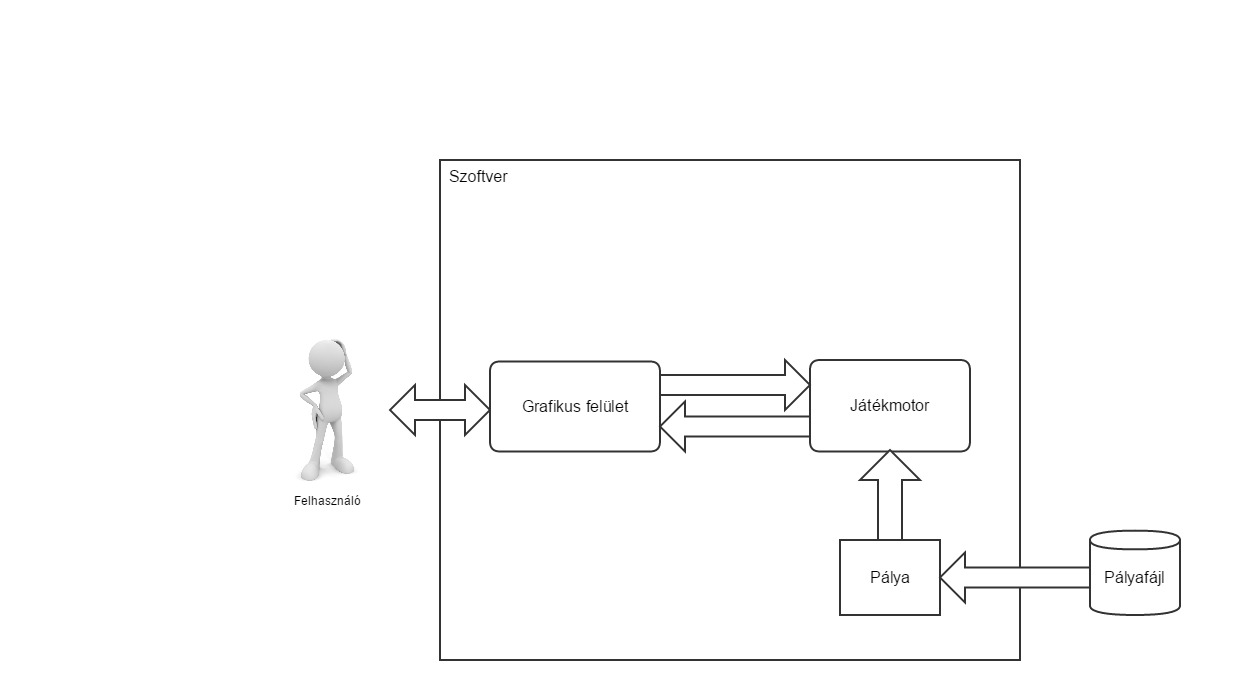
\includegraphics[width=180mm, center]{./chapters/chapter02/dia1.jpg}
	\caption{Architekturális kép \label{overflow}}
\end{figure}

A szoftverünk legfontosabb komponense a játékmotor. Itt zajlanak le a számítások, ez futtatja a logikát, ami érzékeli, hogy egy robot elhagyta a pályát, esetleg beleugrott egy ragacsba, vagy egy olajfoltba. A játékmotor feladata az is, hogy észrevegye, amikor vége van a játéknak, azaz lejárt az idő, vagy csak egy robot maradt a pályán. \\

A grafikus felület a felhasználó számára megjeleníti a játékot, valamint ezen keresztül tudja befolyásolni a játékmotorban történő eseményeket. \\

Az előre elkészített pályát egy külső fájlból érjük el, ezt tartja nyilván a Pálya modul. A játékmotor természetesen hozzáfér ehhez, hiszen neki kell eldöntenie a robotok kezdőpozícióját, valamint az előre legenerált ragacsok és olajfoltok elhelyezkedését. \\


%Ennek kell 4000 karakternek lennie, ennek a követelménynek megfelel. Ennek az az ára, hogy tűnhet neekd is úgy, mint ha 1-2 dolog ismtlődne benne. No ezt azzal védeném, hogy van például egy rovid kis bevezető (1. bekezdés), ott van néhány dolog említve nagyjábókl a játékról, s utána ezeket kifejtem kicsit bővebben, ezért tűnhet úgy az ismétlés. A mennyiséget nem igen kéne csökkenteni, ahol nagyon rossznak érzed, azt kérlek bommierenben próbáljuk meg megvitatni, s igyekszem megvédeni. Fogalmazási kuszaságok vannak benne bőven, azt javítsátok bátran, ha valami nagyon feltűnően rossz, azt szintén említsétek, hogy tanuljak belőle. - sgabor
\subsection{Funkciók}

A szoftver egy úgynevezett Phoebe versenyszimulátor, amelyben robotok versenyezhetnek egymással. Először álló helyzetből indulnak, mindegyik egy előre generált pozícióból. A játék körökre osztott. Minden kör egy iterációnak felel meg, így minden játékos egy körben maximum két dolgot tehet meg: ragacsot helyezhet el, vagy olajfoltot hagyhat maga után (a kettő közül természetesen csak az egyiket), valamint változtathatja a sebességét. A robotok egy előre elkészített versenypályán mozognak. A pályáról leugró robotok elakadnak és kiesnek a játékból.\\

A robotok sebessége egységnyi méretű, tetszőleges irányú sebességvektorral tetszőlegesen módosítható. Egy ugrással a sebességgel egyenesen arányos távolságra tudnak eljutni.\\

Az elején betöltődik a pálya, ami szabályos sokszögekből fog állni, majd véletlenszerűen generálódik rá néhány olaj -és ragacsfolt, valamint a játékosokhoz tartozó robotok. A játék csak többjátékos módban játszható és minden körben szépen sorban mindenki beállíthatja, hogy merre kívánja módosítani a robotjának a sebességét, és hogy kíván-e hátrahagyni valamilyen foltot. Ezután a megadott beállítások végrehajtódnak, s ennek megfelelően ugrik egyszerre az összes robot. Ha két robot ugyanarra a mezőre ugrik, akkor mindkettőt eldobja a játék egy véletlenszerű üres szomszédos cellába, ha pedig ez nem lehetséges (mert a pálya széle, vagy az őket körülvevő robotok akadályozzák ebben), tehát ha nincs két szabad cella az adott cella körül, akkor mindkét robot megsemmisül és ezáltal kiesik a játékból.\\

Ha a robot olyan cellába ugrik, ahol már nem tart a pálya, akkor leesik és szintén kiesik a játékból. Ha már csak egy robot marad a pályán, akkor játék véget ér és az egyetlen fennmaradó robot irányítója nyert.\\

A játékot a következő sebességre hatással bíró funkciók nehezítik meg, s teszik izgalmassá a versenyzést: a pályán vannak olajfoltok, amikre érkezve sebességmódosításra nincs mód, illetve ragacsfoltok, amik a sebesség nagyságát megfelezik. A robotok fel vannak szerelve olaj és ragacskészlettel, amiket a játékos parancsára elugráskor maguk mögött tudnak hagyni. Amelyik robot a legügyesebben gazdálkodik ezekkel a képességekkel, az nyilván könnyen előnyre tehet szert az ellenfeleivel szemben, garantálva a szórakozást. Összefoglalva a pályán keletkező lehetséges akadályok és az egyéb verseny kimenetelére hatással bíró tényezők a következőek:\\

\begin{itemize}
	\item Olajfolt: hatására a robot sebessége nem módosítható, azaz a következő ugrás sebességvektora meg fog egyezni az előző ugráséval, ami a pályaelhagyáshoz vezethet, ami a robot számára a játék végét jelenti.
	
	\item A másik lehetséges folt a ragacs. Ez minden esetben megfelezi a robot sebességét, tehát lassító hatással bír. Az idő lejártához közeledve nyilvánvaló, hogy a ragacsba való belépés akár az első hely elvesztésével is járhat, ezért célszerű elkerülni.
	
	\item Lyukak: a pályán véletlenszerűen lyukak lesznek találhatóak, a pálya generálásának véletlenszerűségéből adódóan (a pálya nem feltétlen egy szabályosnak mondható alakzatot vesz majd fel, így szélein is egyenetlenségek keletkezhetnek majd). Ezekre a lyukas cellákra lépve a játék az adott robot számára szintén véget ér.
\end{itemize}

Mindenkinek lesz korlátozott számú foltja amit a pályára dobálhat. Egy cellán csak egyféle folt lehet, vagy üresen is állhat természetesen. Foltot már az első kör végén is hagyhatnak maguk után a robotok. A folt hatása csak addig tart, amíg a robot el nem lép a "foltos" celláról. Ha egy robot belelép egy foltba, akkor a folt nem tűnik el, hogy később más is beleléphessen, így a foltos cellák száma sosem csökkenhet, ezzel is fenntartva a játék izgalmait.\\

Az olajfoltot vagy a ragacsot az ugrás előtt tudja maga mögött hagyni, természetesen ezt a felhasználó dönti el, hogy mikor alkalmazza. Legcélszerűbb akkor kiadni ezeket az utasításokat, amikor az ellenfél nagy eséllyel nem, vagy csak nehezen tudja elkerülni az ezen való áthaladást.\\

A játékot a következőképpen lehet megnyerni: az ellenfelek a fent leírt okok valamelyike miatt megsemmisülnek, s már csak egyetlen robot marad fenn a pályán; vagy az a robot nyer, amelyik a megadott idő -illetve körlimit letelte után a legnagyobb utat tette meg.\\

\subsection{Felhasználók}

A szoftver több felhasználóra van tervezve, akik számára a játék könnyedén elsajátítható, amennyiben ismerik a szótárban megnevezett definíciókat. Egyjátékos módra nincs lehetőség.

\subsection{Korlátozások}

Korlátozásként megfogalmazható az, hogy a forrásprogramnak a laboratóriumban rendszeresített JDK alatt lefordíthatónak és futtathatónak kell lennie, nem adható hozzá külső package.

\subsection{Feltételezések, kapcsolatok}

Szoftver labor 4 feladatkiírás: \textit{https://www.iit.bme.hu/$\sim$szoftlab4/feladat.shtml}